\documentclass{article}
\usepackage[UTF8]{ctex}
\usepackage{geometry}
\usepackage{natbib}
\geometry{left=3.18cm,right=3.18cm,top=2.54cm,bottom=2.54cm}
\usepackage{graphicx}
\pagestyle{plain}	
\usepackage{float}
\usepackage{setspace}
\usepackage{caption2}
\usepackage{datetime} %日期
\renewcommand{\today}{\number\year 年 \number\month 月 \number\day 日}
\renewcommand{\captionlabelfont}{\small}
\renewcommand{\captionfont}{\small}
\begin{document}

\begin{figure}
    \centering
    
\includegraphics[width=8cm]{upc.png}

    \label{figupc}
\end{figure}

	\begin{center}
		\quad \\
		\quad \\
		\heiti \fontsize{45}{17} \quad \quad \quad 
		\vskip 1.5cm
		\heiti \zihao{2} 《计算科学导论》课程总结报告
	\end{center}
	\vskip 2.0cm
		
	\begin{quotation}
% 	\begin{center}
		\doublespacing
		
        \zihao{4}\par\setlength\parindent{7em}
		\quad 

		学生姓名:\underline{\qquad  张航 \qquad \qquad}

		学\hspace{0.61cm} 号:\underline{\qquad 1907010218\qquad}
		
		专业班级:\underline{\qquad 计算1902 \qquad  }
		
        学\hspace{0.61cm} 院:\underline{计算机科学与技术学院}
% 	\end{center}
		\vskip 2cm
		\centering
		\begin{table}[h]
            \centering 
            \zihao{4}
            \begin{tabular}{|c|c|c|c|c|c|c|}
            % 这里的rl 与表格对应可以看到,姓名是r,右对齐的;学号是l,左对齐的;若想居中,使用c关键字。
                \hline
                课程认识 & 问题思 考 & 格式规范  & IT工具  & Latex附加  & 总分 & 评阅教师 \\
                30\% & 30\% & 20\% & 20\% & 10\% &  &  \\
                \hline
                 & & & & & &\\
                & & & & & &\\
                \hline
            \end{tabular}
        \end{table}
		\vskip 2cm
		\today
	\end{quotation}

\thispagestyle{empty}
\newpage
\setcounter{page}{1}
% 在这之前是封面,在这之后是正文
\section{引言}
计算机科学与技术发展至今,也算是度过了七十余年的时间。计算机也由最初的各种问题,如:1、它是个庞然大物,用了18000个电子管,占地150平方米,足有两间房子大,重达30吨,耗电功率约150千瓦,每秒钟可进行5000次运算。2、由于它使用的电子管体积很大,耗电量大,易发热,因而工作的时间不能太长。3、使用机器语言,没有系统软件,因此操作起来很麻烦。4、采用磁鼓、小磁芯作为储存器,存储空间有限,所以不能用来做大量运算,因此它的作用并不算太大。\par
\begin{figure}[h!]
	\centering
	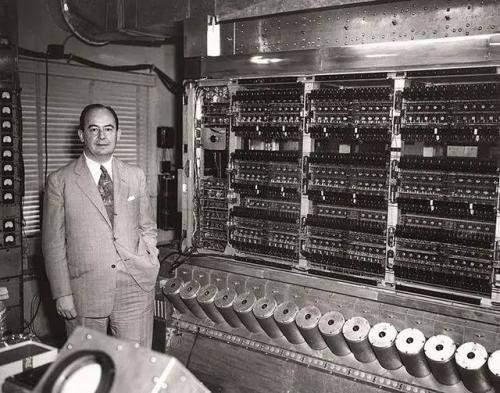
\includegraphics[scale=0.7]{jisuanji}
	\caption{世界上第一台通用计算机和它的制造者冯·诺伊曼}
	\label{fig:jisuanji}
\end{figure}
但经过这七十多年的发展,计算机的发展可以说是飞一般的变化。经过像小孩子一样笨拙但又不停地前进,如今,计算机的发展可以说是有了质的飞跃。新时期的计算机体积、功耗、重量进一部减小,运算速度、存储容量、可靠性都有了很大的提高。计算机更是给人类社会带来了极大的变革。如今,计算机已成为人类社会所必不可少的工具之一,人们的生活也几乎离不开计算机的应用。\par 
随着我国经济的迅速发展和世界科技的不断进步,我国的计算机科学与技术领域获得了飞速的发展。计算机科学与技术在多个方面获得了充分的利用,教育、经营、管理等多个方面都有所涉及,老师、企业家、政府工作人员都利用计算机科学与技术获得在其工作领域的重要发展。\citep{b}计算机技术已经渗透到了人们生活的方方面面。\par
\begin{figure}[h!]
	\centering
	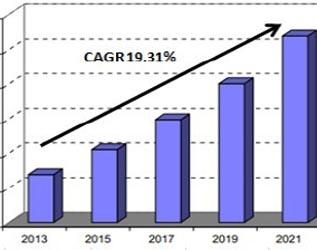
\includegraphics[scale=0.9]{jisuanjifazhanqushi}
	\caption{计算机的发展趋势}
	\label{fig:jisuanjifazhanqushi}
\end{figure}
正是由于如今计算机在人类社会重要的应用,因此我选择了计算机这个专业,更是在计算机导论课上深入了解了计算机这一专业的过去历史,如今现状以及光明未来之后,更加坚定了我投身计算机伟大事业的决心。出于对计算机导论课上所掌握知识的巩固与总结,于是这一篇报告应运而生。对计算机科学导论这门课程的认识与思考以及从中所得到的知识与体会,都将包含在其中,不仅如此,还会有对针对课堂演讲课题的更加深入的思考。\par
除此之外,这篇报告还会涉及在课上演讲的课题的有关内容基因。主要是关于基因测序技术的发展历史及计算机技术在基因测序发展过程中所起的推动作用与如今计算机技术和基因测序的之间的联系。虽然基因测序技术的发展对于普通人而言过于遥远,但它却实实在在的可以改变人类的生活,这是不容置疑的。我个人认为,基因测序技术会与计算机技术一样在未来会普遍地出现在人们的生活中,与计算机技术一样成为人们日常生活的一部分。因为最新研究结果表明:“人类绝大多数疾病都与基因有关,并且可以遗传。人类掌握自身健康命运的梦想正在随着基因功能研究的深入接近现实。”因此,研究基因成为未来医学研究的主要方向,而基因测序技术的应用是必不可少的。而在基因测序技术的发展中,计算机技术在其中也起着至关重要的作用。因此基因测序技术的发展必然与计算机技术相关联。\par

计算机软件分析阿拉伯糖代谢酶C调节蛋白基因(Ara C)以及细胞周期素依赖型蛋白激酶反应蛋白基因(C1P1)的五组重复测序结果,发现该软件不仅能用图示分析方法准确显示编码序列及编码容量,而且其依据生物界密码子偏倚规律,采用比较法评估高频率使用实用型密码子的优质开放读码框架.能使分析者对复杂多量的核酶信息做初步筛选,从而取舍冗余的基因信息.\citep {a}从这段文字中就可以看出,计算机技术在基因测序技术上的巨大作用。让基因测序不再那么难以进行,为基因测序的便捷化、便民化、快速化、高通量化做出了巨大贡献。\par 
\begin{figure}[H]
	\centering
	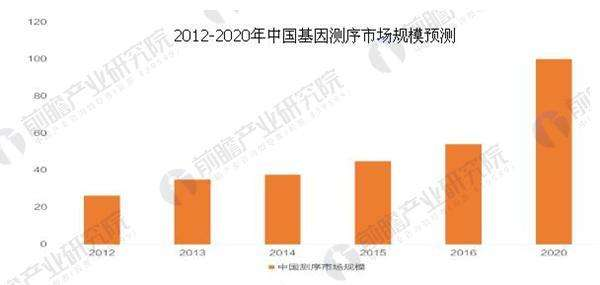
\includegraphics[scale=0.7]{jiyincexushichangguimoyuce}
	\caption{基因测序技术的市场规模及预测}
	\label{fig:jiyincexushichangguimoyuce}
\end{figure}
这就是本次报告所包含的主要内容,希望通过这次报告的撰写,能更加理解这一门课程,更加理解计算机这一专业的深邃。当然,也希望能通过这次报告的撰写,督促自己去了解更多关于计算机科学导论课程的重要性、计算机科学导论课程对于大一新生的重要性以及更多关于计算机的相关知识并掌握这些知识使自己更加充实,从而让这次报告更有价值与意义。\par 

\section{对计算科学导论这门课程的认识、体会}
 
\subsection{关于计算科学导论}
大学计算机课程中的计算机导论课程是作为普通院校计算机专业学生入校后第一个需要学习的基础课程。提出大学计算机课程,不能一味地强调计算机是作为工具使用而存在着,应摒弃计算机科学没有理论只是工具的错误认识,需要将计算思维引入到大学计算机基础课程教学中,可从激发学生学习兴趣为导入,以直观教学为基点,以团队协作为支撑,以重视实验及作业为重要辅助的计算机导论教学方式。形成围绕使用计算手段求解问题的全过程来指导学生学习该课程进行了探讨。\par
一直以来,计算科学导论作为当代大学计算机科学与技术专业中一门颇有争议的课程,在计算科学教育界一直存在着认识上的分歧,包括是否需要开设这一门课程,如果开设这一门课程,那对于这门课程而言应该按排多少学时,在这门课程讲授过程中又应该以什么为重点等等一系列问题。但是根据“教育部计算机科学类专业面向21世纪教学内容与课程体系改革课题(13-22)”研究工作的进展和体会而言,我认为在计算机科学与技术专业第一学期中开设这一课程是很有必要的。\par 
就目前而言,虽然绝大多数学校自从二三十年前就开设了这一门课程,但随着教育界对于计算机科学与技术专业教育认识的不断深化,原有教材的缺点暴露无遗:\par 
1、大多数《计算科学导论》教材在内容上写成了计算机科学与技术专业基础课程的一个压缩版。\par 
2、导论的内容与后续课程的衔接缺乏科学的论证。由于一年级学生尚缺乏学习后续课程必要的基础知识,因此该课程便承担了一些本来应该由其他课程承担的教学内容。\par 
然而,赵致琢先生所出版的《计算科学导论》一书却完全没有这些偏差,赵致琢先生总结了以前课程版本的不足并结合现在的课程要求,从而编写了这部符合学生的认知实际与课程要求的教材,是很适合我们大一新生学习的。\citep{f}\par 
每一门课程总有其存在的意义,计算科学导论的存在更是计算机科学与技术专业极其重要的一门课程。计算科学导论更应该就学科特点、学科形态、历史渊源、发展变化、典型方法、学科知识组织结构和分类体系等问题从科学哲学和高年级科普的角度去回答大家关于该学科的疑问,而不是添加各种应该由以后课程讲授的知识。计算科学导论更像是一个引路人,在一开始就告诉你你将来需要学习的内容并且培养学生计算科学的思维。引导你去认识自己将来需要面对的,并给出关于你的选择的建议,避免少走弯路。\par 

\subsection{ 对计算科学导论的认识与体会
}
“什么是计算?我相信,世界上没有两个计算机科学家会就这一概念给出相同的定义。”由此可以看出计算复杂性。而计算科学呢?计算科学又是什么呢?\par 
计算科学是对描述和变换信息的算法过程,包括其理论、分析、设计、效率分析、实现和应用的系统的研究。全部计算学科的基本问题是,什么能有效地自动进行,什么不能有效地自动进行。计算科学导论更应该成为一个指路人,指导学生去了解学科特点,了解学科的发展历史。\par 
可能很多人认为,计算科学导论就是一门水课,随便混混就可以。但是,大学里开设的每一门课程都是有它的意义的。计算机导论大多数在大一第一学期开设,主要用来介绍计算机科学体系的方方面面,包括操作系统,组成原理,网络,数据库,数据结构与算法的基础性概念,软件工程,安全等知识,能够帮助建立计算机科学的学科体系,强烈建议学习,提纲挈领的作用。计算科学导论课程的重要性不言而喻。\par 
计算机导论课是为了让我们学习计算机本科专业的新生提供关于计算机学科的入门介绍。当我们对于学习计算机迷茫不知所措时,计算机导论课为我们指明方向。随着科学技术的发展,信息时代的到来,人类各种知识的爆炸式增长,我们已经不得不承认计算机已经成为我们人类社会的基石,已经悄无声息的渗透到我们生产生活的各个方面,巨大的影响并推动我们人类社会的发展。人类社会已经无法离开计算机,我们也应该对其有一定的认识。而对于计算机的这些认识,便是我在计算科学导论课程上所获得的最为重要的知识。\par 
首先,计算科学导论为我们全面介绍了计算机的基本知识、硬件系统、软件开发、数据库基础、计算机网络与安全、计算机的应用技术以及计算机文化等。一开始,老师向我们介绍了计算机的发展史,并且让我们知道了计算机从简单的计算需求到后来的文字处理,人工智能等,几乎服务于各行各业。并向我们介绍了如今计算机网络公司的工作环境和和薪资问题,并展示了公司的工作环境。鼓励我们投身于计算机事业。\par 
其次,还向我们介绍了计算科学的意义、内容和方法。包括什么是计算科学、学科目前的基本问题以及计算科学的发展主线。而最重要的是计算科学的分类与分支学科简介。原本以为计算科学只是单纯的一门技术,但在上完了计算科学导论课,才知道了计算科学竟然也分如此多的种类:\par 
1、离散结构(DS)\par 
2、编程基础(PF)\par 
3、算法及复杂性分析(AL)\par 
4、组织和体系结构(AR)\par 
5、操作系统(OS)\par 
6、以网络为中心的计算(NC)\par 
7、编程语言(PL)\par 
8、人机交互(HC)\par 
9、图形及可视化技术(CV)\par 
10、智能系统(IS)\par 
11、信息管理(IM)\par 
12、社会及职业问题(SP)\par 
13、软件工程(SE)\par 
14、计算科学与数值计算法(CN)\par 

\subsection{从计算可视化浅谈对计算科学导论的认识与体会}
我们都知道,计算机应用和计算机基本应用技术是一回事,涉及到的分支学科很多。然而,从计算机应用的定义和科学方法论的角度出发,大致可以将计算机应用分支学科的范畴确定下来,即它所研究的内容在方法和技术上为计算机在各个领域的具体应用奠定了基础。\par 
按照这样的定义,计算机应用主要包括数值计算,信号处理技术,图形学与图像处理技术,网络技术,多媒体技术,计算可视化与虚拟现实技术等等方面,而计算可视化就是我要说的重点。\par 
1、什么叫可视化?\par 
科学计算可视化(Visualization in Scientific Com-puting)是发达国家八十年代后期提出并发展起来的一门新兴技术。它将科学计算过程中及计算结果的数据转换为几何图形及图象信息在屏幕上显示出来并进行交互处理,成为发现和理解科学计算过程中各种现象的有力工具。 科学计算可视化将图形生成技术和图象理解技术结合在一起,它既可理解送入计算机的图象数据。也可以从复杂的多维数据中产生图形。它涉及到下列相互独立的几个领域:计算机图形学、图象处理、计算机视觉、计算机辅助设计及交互技术等。实际上,目前科学计算可视化技术已经不仅用于显示科学计算的中间结果和最终结果,而且还用于工程计算及测量数据的显示。\citep{c}\par
2、可视化的发展历史\par
 计算机用于科学计算已有40多年的历史。在20 世纪50年代和60年代,由于计算机的硬件、软件技术水平的限制,科学计算只能以批处理方式进行,大量输出数据的解释与理解所花费的时间往往是计算时间的十几倍甚至几十倍,这一阶段谈不上科学计算的可视化。70年代以后,虽然可以将科学计算的结果以二维图象表示,用绘图仪绘制出来,但仍然不能得到计算结果的直观、形象的整体概念,而且不能进行交互处理,只能被动地等待计算结果的输出。\par 
 近年来,随着科学技术的迅猛发展待处理的数据量越来越大,来自巨型计算机,地球卫星、宇宙飞船、计算机断层摄影(CT)扫描仪及地震勘测的数据与日俱增,原有的数据处理及显示手段远远不能满足要求。在这样的形势下,1987 年2月美国国家科学基金会在华盛顿召开了有关科学计算可视化的首次会议,与会者有从事计算机图形学、图象处理及各种不同领域科学计算的专家,会议一致认为: 将图形和图象技术应用于科学计算,这是一个全新的技术领域, 会议将这一技术定名为科学计算可视化。\par 
 国内仅有少数单位在进行科学计算结果数据可视化技术的研究,少数拥有较强计算能力的计算中心正开始应用这一技术实现有关领域的可视化,如气象、计算流体力学、天文、生物化学等。在美国等发达国家的超级计算中心、国家实验室、著名大学里,则已在超级计算机、光纤网、高档工作站的环境中实现了计算流体力学、有限元分析、医学图象、天体物理等领域计算结果的实时跟踪处理及显示,并正在研究科学计算过程的交互控制技术。已有商品化的科学计算可视化软件提供给用户使用,如 AVS 等。\par 
 3、计算可视化与计算科学导论\par 
  计算可视化的应用方面很多,如数据可视化、疾病诊断、地质勘探、气象预报、分子模型构造、计算流体力学、有限元分析、基因测序等方面。不仅如此,
  Ravil I. Muhamedyev,Y. Daineko曾在他的一篇文章里用对分子复合模型的展示指出,可视化不仅可以定性化,还可以进行定量化分析:“ A method for three-dimensional visualization of molecular biology processes modeled by chemical kinetic equations is presented. To implement this visualization, the software in C++ and a database of three-dimensional forms that model molecular complexes are developed. The quantitative parameters in this visualization scheme are determined from kinetic equations governing the participating components, so our visualization is not only qualitative but also quantitative. As a case study, it was visualized a mathematical model for mitochondria-dependent apoptosis (programmed cell death) proposed by Bagci et all ”。\citep{e}这分别都归为不同的研究方向,因此想要向学生介绍完这些显然是不现实的。这里便体现了计算科学导论课程的学科特点了。提到但不深入,涉及但不重点考虑。只是对其作一个基本的介绍,让学生知道了解。计算可视化是一个研究方向,是计算科学导论中的一个点。从计算可视化这一方面的研究来看,计算科学导论更能体现一个引路人的角色定位,它更像是一个经验丰富的人,在向我们这些新生小白介绍自己的经验,让我们能提前了解这个大千的世界,去为自己的人生早做准备。\par 

\section{进一步的思考:计算机在基因测序中的作用}
在课堂分组演讲中,我和同伴就基因测序的原理、发展历程、成就及目前的发展趋势进行了一次演讲,但由于在分组演讲中对主题理解有一定的偏差,因此在演讲过程中关于计算机与基因测序方面的联系讲述并不多这里就基因测序与计算科学知识之间的联系做一些阐述。\par
施一公先生曾在清华大学说过“21世纪是生物学的世纪”。足以看出生物学在本世纪的重要性与发展的前景,而基因测序的作用更加明显。因为“绝大多数的病都是基因病”。这一论断使得基因诊断在治病的过程中更加重要,因此,测定基因序列便成为一项至关重要的事情。基因测序已经在很多地方有了实质性的进展。\par 
  
  Ying Qian,Yu Zhang,Bingyu Guo  在他们的关于基因启动子的论述中,曾指出“Gene expression is regulated by transcription and translation, and the promoter controls the start of transcription. Finding the exact location of a promoter is of great importance to life science. With the development of the Next-Generation Sequencing (NGS), more and more eukaryotic gene sequence data are available. Computational prediction of eukaryotic promoters has become one of the most challenging problems in sequence analysis. Many methods have been proposed, but the accuracy of prediction still needs to be improved. In this paper we use support vector machine (SVM) to verify that promo”\citep{d}启动子在基因诊治中如此重要,却因序列复杂而难以确定。这不正是计算机的长处所在?大数据的处理能力使得计算机能够在这方面发挥极大的作用。\par 
Fox, E. J.和Loeb, L. A在他们的One cell at a time一文中提到“Single-cell DNA sequencing of two breast-cancer types has shown extensive mutational variation in individual tumours,confirming that generation of genetic diversity may be inherent in how tumours evolve.”这一研究更是体现了基因测序的重要的作用。由此,在其中起重要作用的计算机技术无疑也是极为重要的。提到测序与计算机的联系,想到最快的无疑是数据的处理与呈现。正是这样,虽然测序中也有其他计算机技术的应用,但就此而言数据处理与呈现以及数据比对却是更重要的。众所周知,基因是极其复杂的,基因的个数是多不胜数,因此在测序过程中,对于测序结果的处理与呈现就显得极为重要。人工来做的话,无疑是一个极大的工作量。而对于大数据处理,这却正是计算机的长处所在。因此,在基因测序的过程中,计算机技术的应用无疑会极大地降低成本,并且让测序技术的发展更加亲民,方便。从而让基因测序技术也能成为一项普及的事物,人人皆可使用。\par 
\begin{figure}[h!]
	\centering
	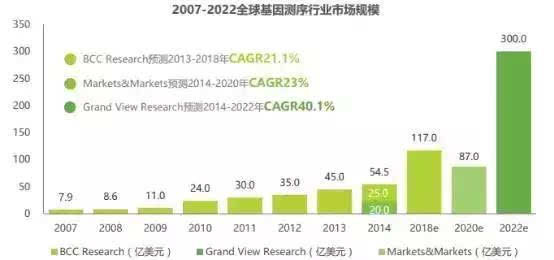
\includegraphics[scale=0.7]{shijiecexuguimoyuce}
	\caption{全世界基因测序的市场规模及预测}
	\label{fig:shijiecexuguimoyuce}
\end{figure}




\section{总结}
通过本学期计算导论课程的学习,我深入了解了计算机行业目前所面临的大的趋势,更有计算机领域的大量常识性内容。计算科学导论不是一门无用的学科,而是一门总结了计算科学领域大量的知识方面的拓展,而这正是大一新生能所需要的。大一新生一般对计算机领域的了解并不多,而计算科学导论这一门课程便正是用来弥补这些缺失与不足的。计算科学导论是一个指路人,在我们尚且一无所知的时候,告诉我们所面临的所有选择,并帮助我们了解这些方向,去了解,去认识,去探索我们感兴趣的方面。从而为我们之后的发展定下坚实基础,让我们能够以此更上一层楼。不仅如此,计算科学导论这一门课更是向我们展示了计算机领域的发展与前景,让我们知道了计算机目前的发展趋势,从而鼓励我们好好学习其他基础理论学科,扎实自己,充实自己,鼓励我们投身于计算机事业的发展。不仅仅是为了在将来能找一个好工作。计算机技术必定是改变人类历史的一项技术。虽然它的发展有兴起有衰落,但如今它却是处于一个极好的时代,一个能够改变人类生活方式的时代。如今计算机行业兴起势头正猛,身为计算机专业的一名学生,我有必要为了计算机事业的继续蓬勃发展贡献上自己一份微薄的力量,让计算机真的造福于世界人民,让人类迈入更加便捷与幸福的时代。\par


\section{附录}

    \begin{figure}[H]
    	\centering
    	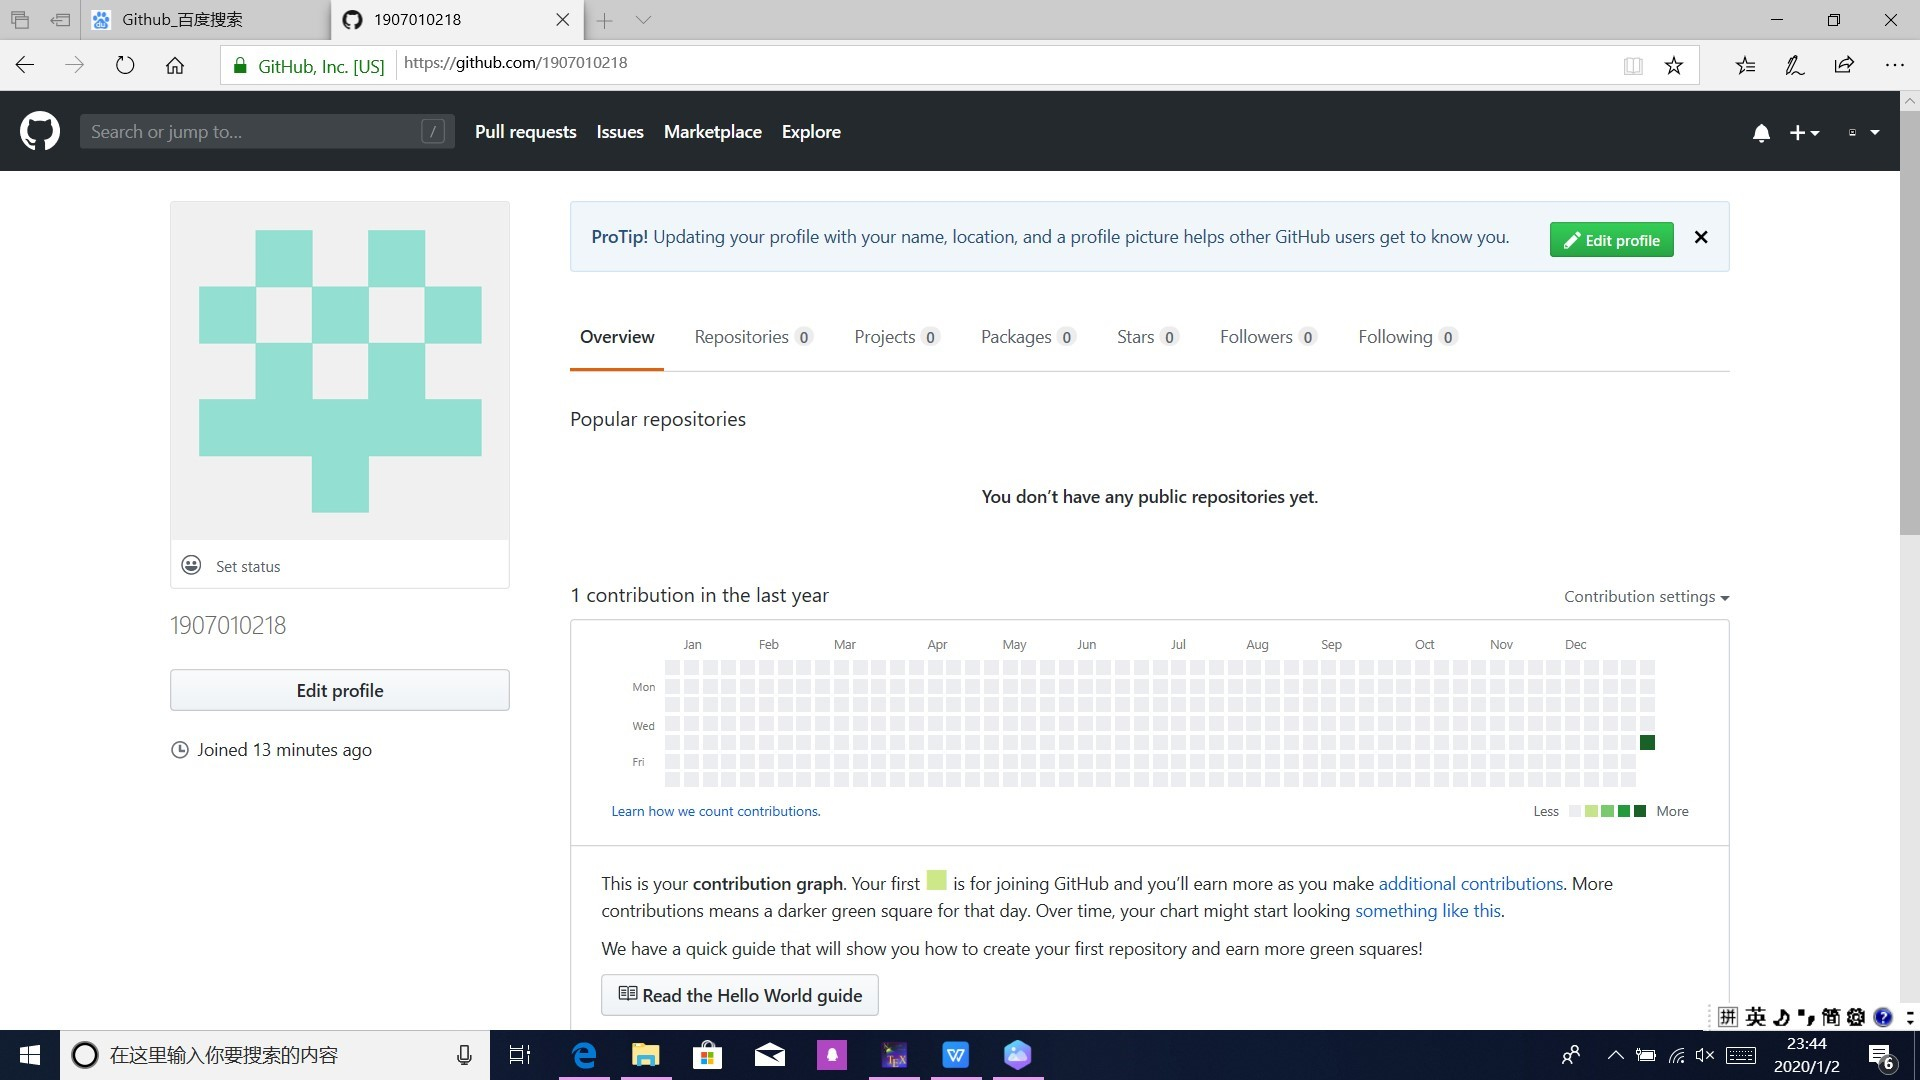
\includegraphics[scale=0.4]{githup}
    	\caption{}
    	\label{fig:githup}
    \end{figure}
      \begin{figure}[H]
    	\centering
    	
\includegraphics[scale=0.3]{bilibili}
    	\caption{}
    	\label{fig:bilibili}
    \end{figure}
  \begin{figure}[H]
	\centering
	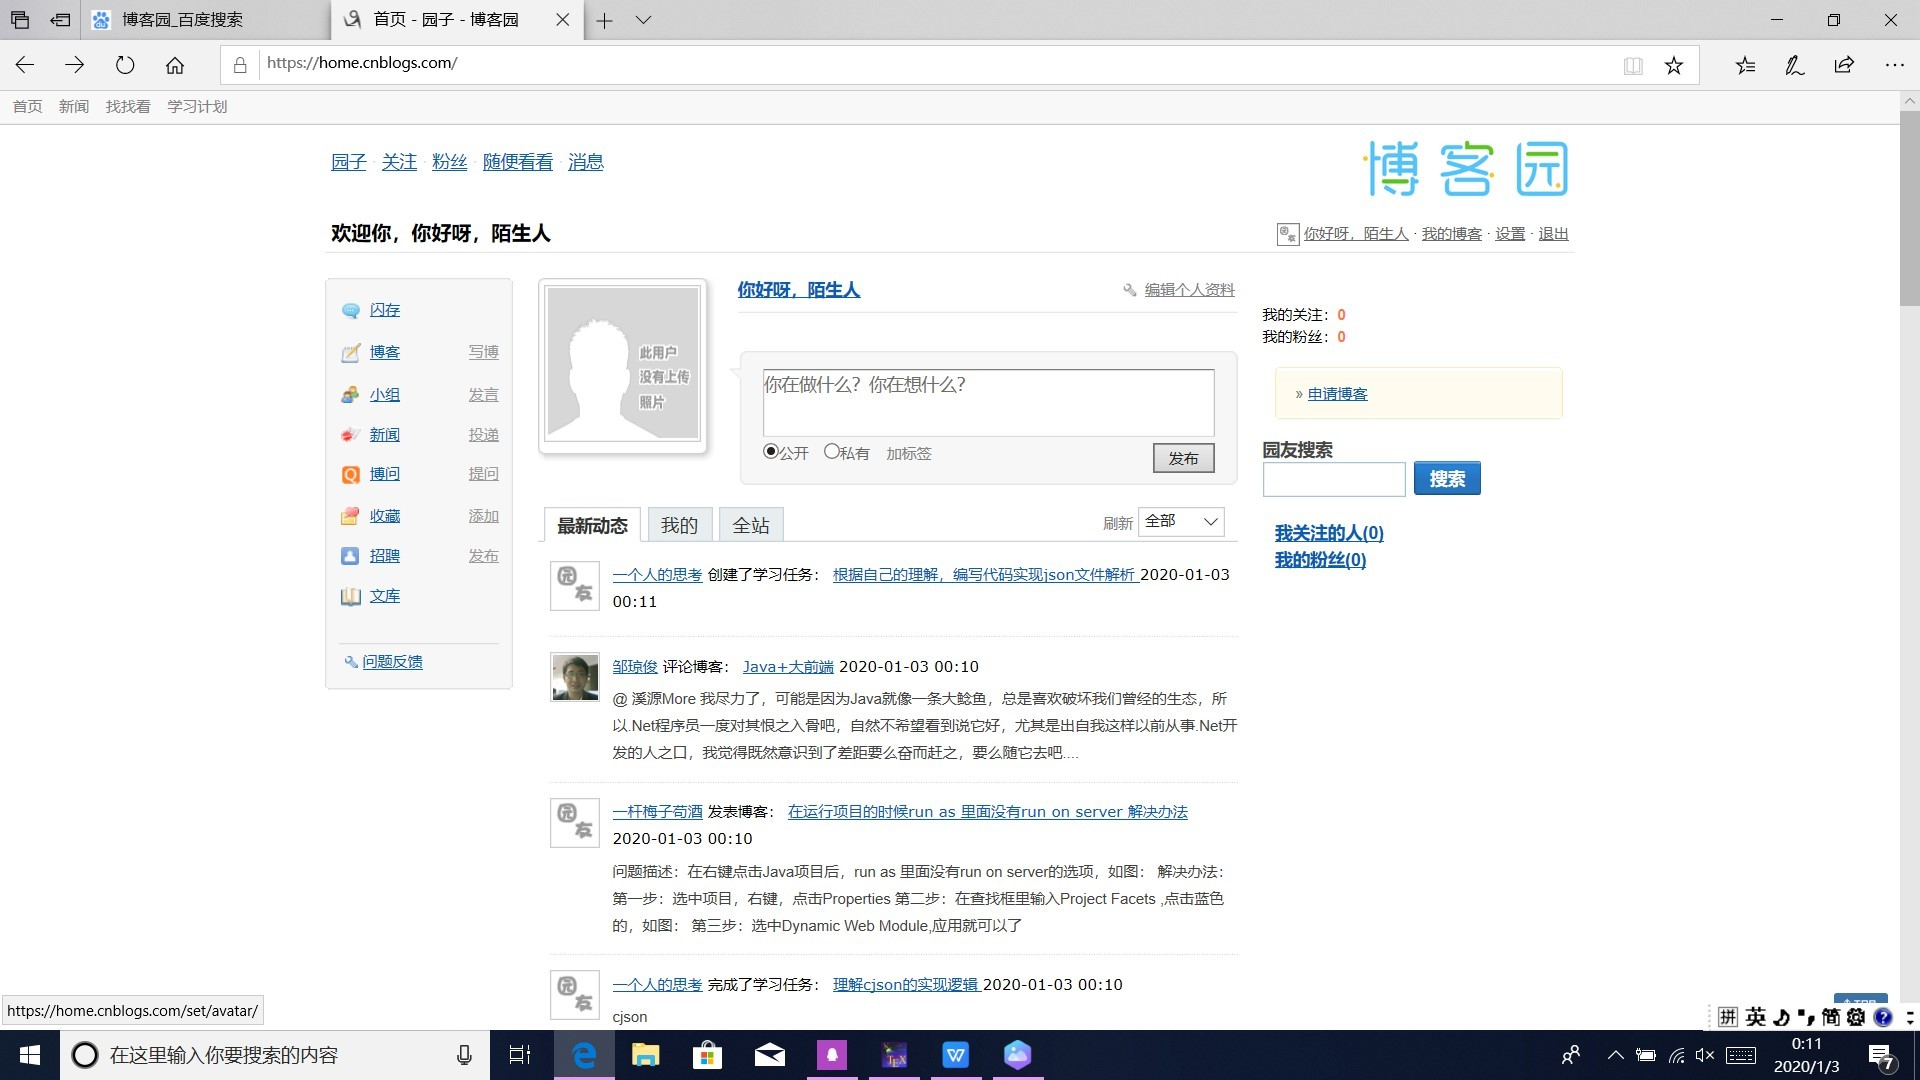
\includegraphics[scale=0.5]{boke}
	\caption{}
	\label{fig:boke}
\end{figure}
  \begin{figure}[H]
	\centering
	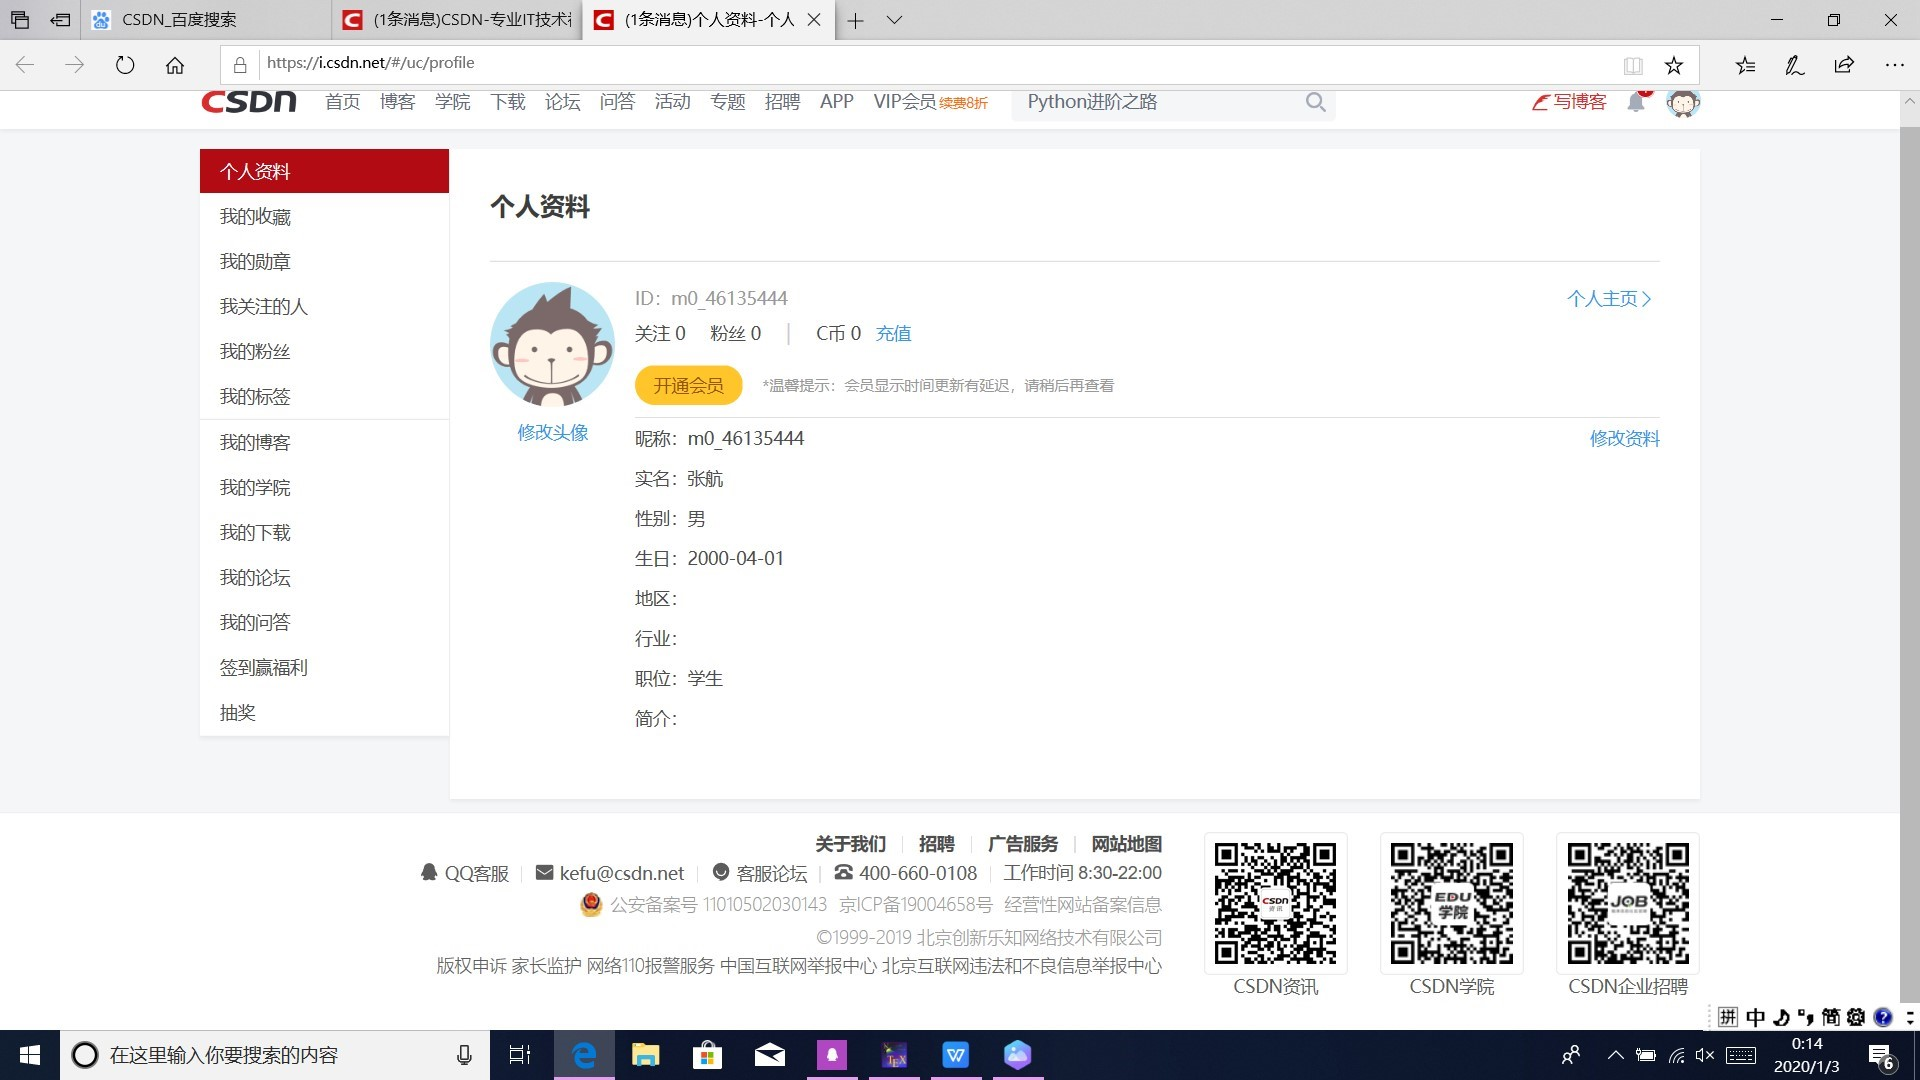
\includegraphics[scale=0.5]{csdn}
	\caption{}
	\label{fig:csdn}
\end{figure}
  \begin{figure}[H]
	\centering
	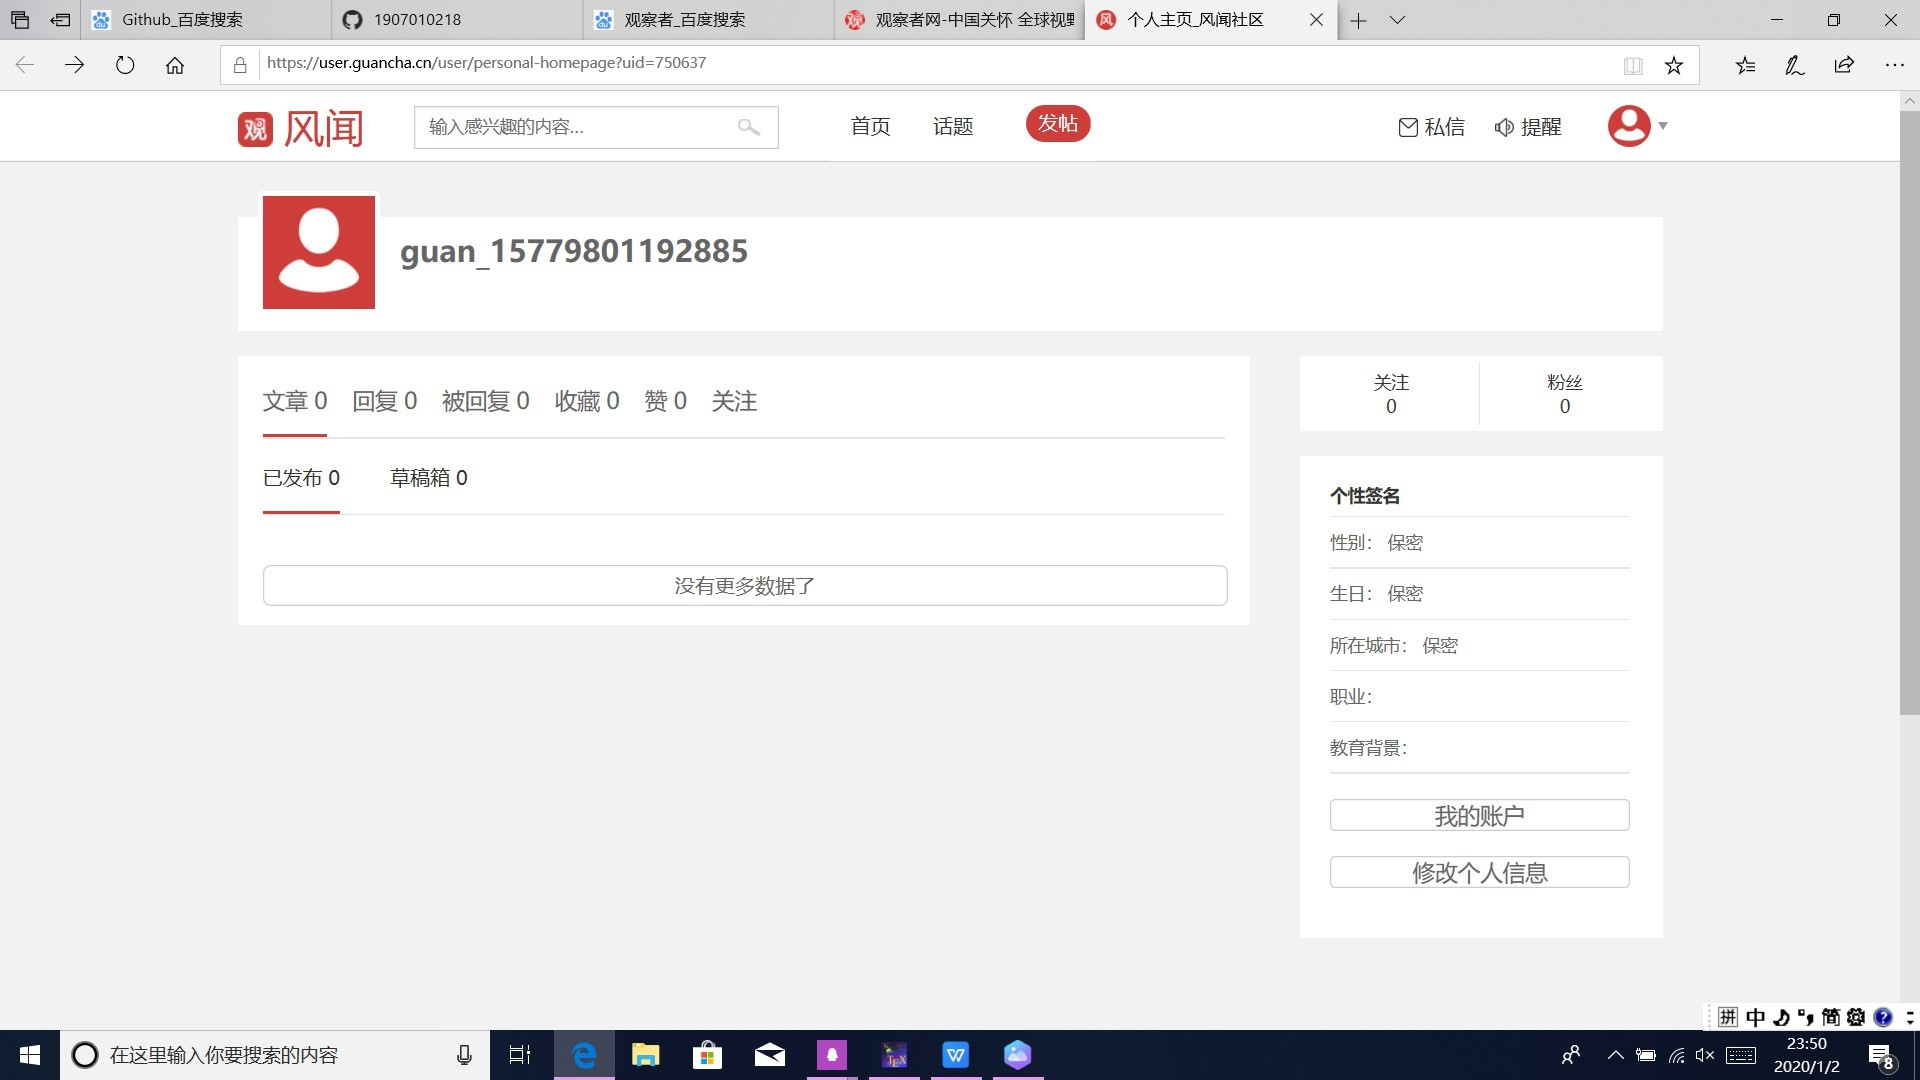
\includegraphics[scale=0.5]{guanchazhe}
	\caption{}
	\label{fig:guanchazhe}
\end{figure}
  \begin{figure}[H]
	\centering
	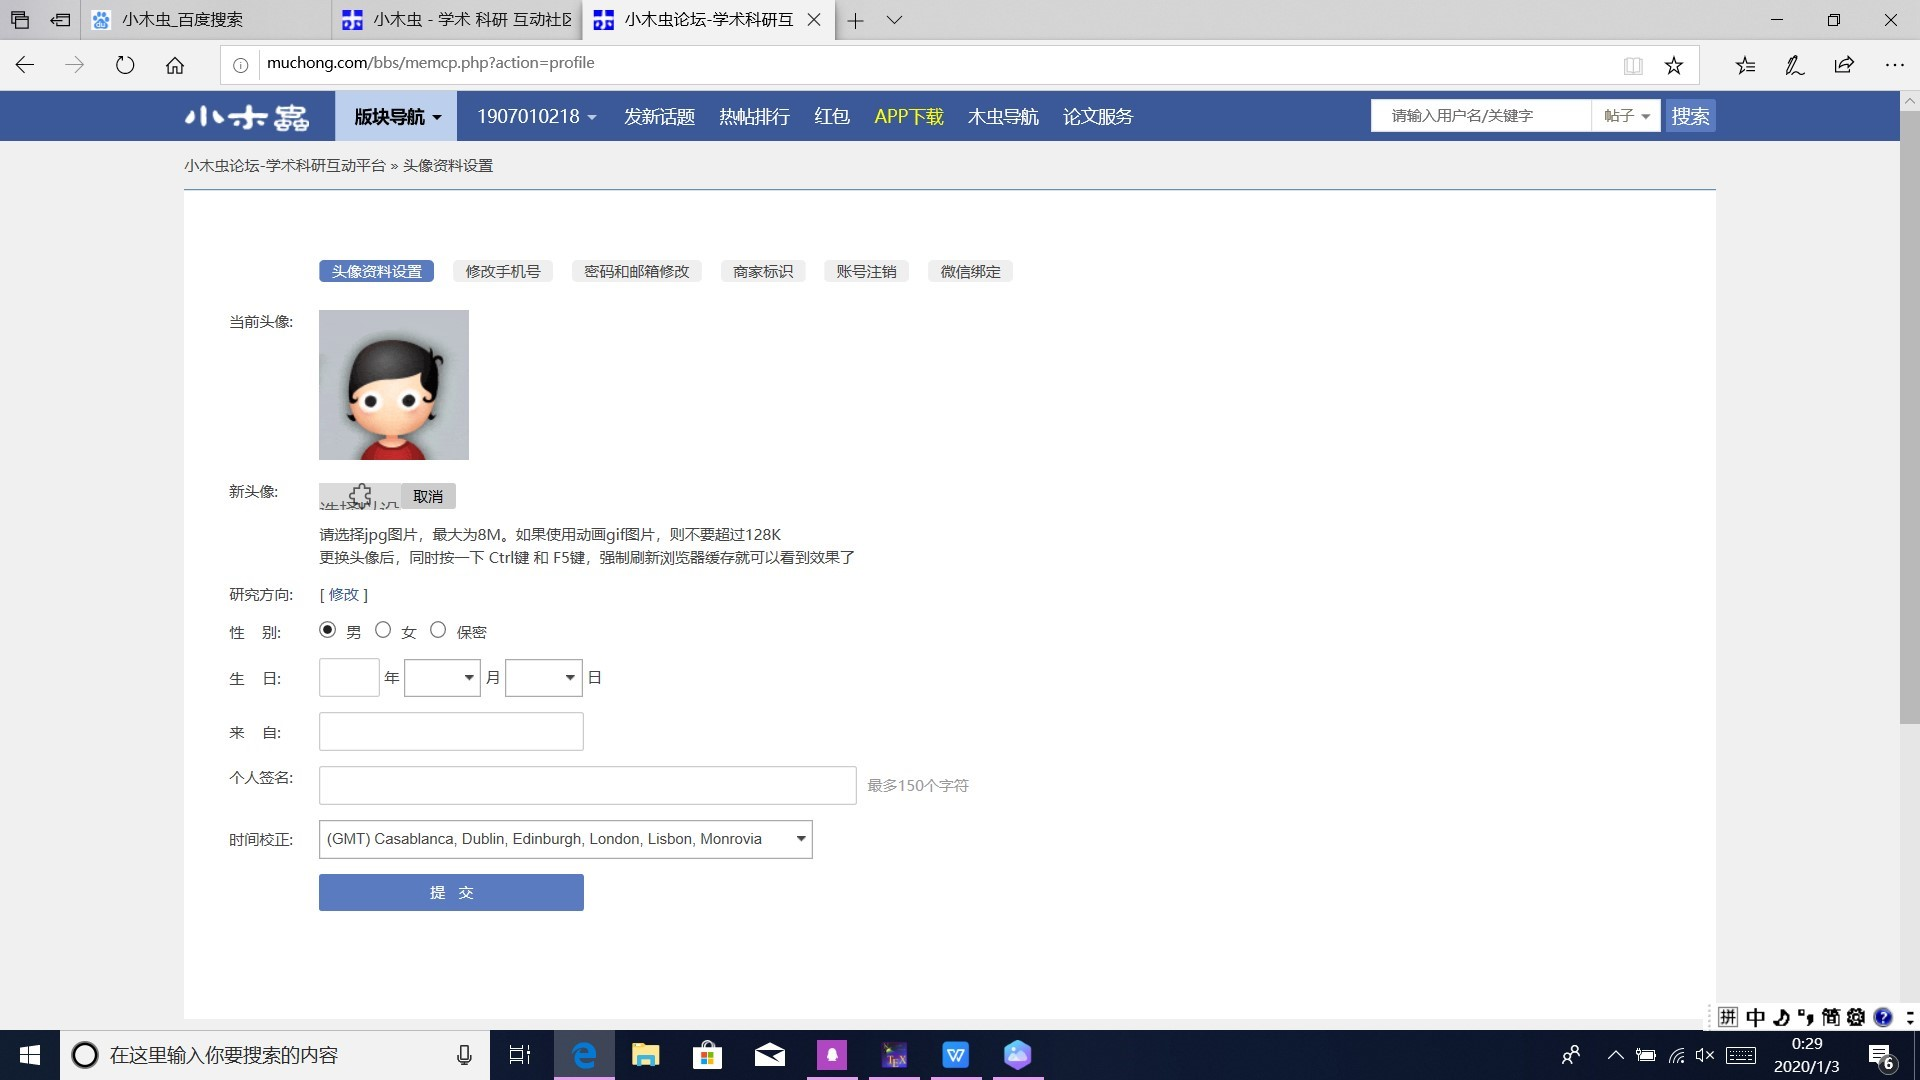
\includegraphics[scale=0.5]{xiaomuchong}
	\caption{}
	\label{fig:xiaomuchong}
\end{figure}
  \begin{figure}[H]
	\centering
	
\includegraphics[scale=0.5]{xuexi}
	\caption{}
	\label{fig:xuexi}
\end{figure}
\hspace*{\fill} \\

{\bf }
\bibliographystyle{unsrt}
\bibliography{references}


\end{document}
